% Generated from paper/source. Do not edit by hand.
\section{NeuroWorld}
\subsection{Causal simulator}
NeuroWorld is a synthetic environment for testing diagnostic reasoning mechanisms without patient data. It defines 20 diagnosis archetypes and 40 findings organized around mechanism, localization, temporality, and context. Each diagnosis specifies factor-dependent finding probabilities, demographic tendencies, and an observation process. Cases are sampled from the causal template, then findings are observed, signed, timestamped, and possibly omitted. The generator emits latent factors so that representation probes and exact interventions are possible.

The simulator is not intended to mimic epidemiology, coding practice, or the full complexity of neurology. Disease names are abstract labels and findings are synthetic variables. “Neurological” describes the structure of the reasoning problem---mechanism, localization, time course, context, and differential competition---not clinical fidelity. The benefit is control: chronology, missingness, nuisance evidence, ambiguity, and new syndromes can be manipulated without harming people or leaking protected data.

\subsection{Chronology twins}
Four labels form two chronology-twin pairs. Members of a pair share aggregate evidence and demographics; two marker events occur in opposite order. Standard random cases may hide one or both markers under the observation process. A separate counterfactual set exposes both markers and varies only order. An unordered model should average the twins and obtain zero pair accuracy in expectation, whereas a valid ordered model can solve both.

Unit tests verify that paired records have equal signed evidence multisets, identical non-temporal covariates, and only the declared ordering difference. Complete-order accuracy is reported separately from all-case top-1. This prevents an architecture from receiving credit for predicting easier factorial cases while ignoring chronology.

\subsection{Factorial diagnoses and held-out composition}
The remaining diagnoses combine mechanism, localization, temporality, and context factors. A held-out composition split removes selected positive-finding conjunctions from training and requires one at test time. The task checks whether a model can recombine familiar individual factors. At 3,000 cases it saturates for several architectures and therefore fails as a discriminator. A stronger future version should reduce data and introduce inseparable tensor or XOR-like interactions with parameter-matched multiplicative controls.

\subsection{Missingness and signed evidence}
Observation is generated explicitly rather than imputing every unobserved finding as negative. Positive findings and observed absences are separate tokens; unobserved findings are omitted. Shift worlds can reduce observation rate, add timestamp jitter, mix probabilities toward 0.5, change nuisance findings, and lower the chance that chronology markers appear. The model is therefore tested both when the causal relation is visible and when the observation process obscures it.

\subsection{Unseen worlds}
The initial shift replication uses a nuisance-seed world and a noisy/sparse world. The confirmation suite declares five unseen world seeds at four severities: nuisance, mild, moderate, and severe. The disease-factor scaffolding remains related, but secondary findings, nuisance evidence, probability noise, sparsity, and temporal jitter vary. These are genuine held-out generator instantiations, though not independently designed simulators.

\begin{figure}[t]
\centering
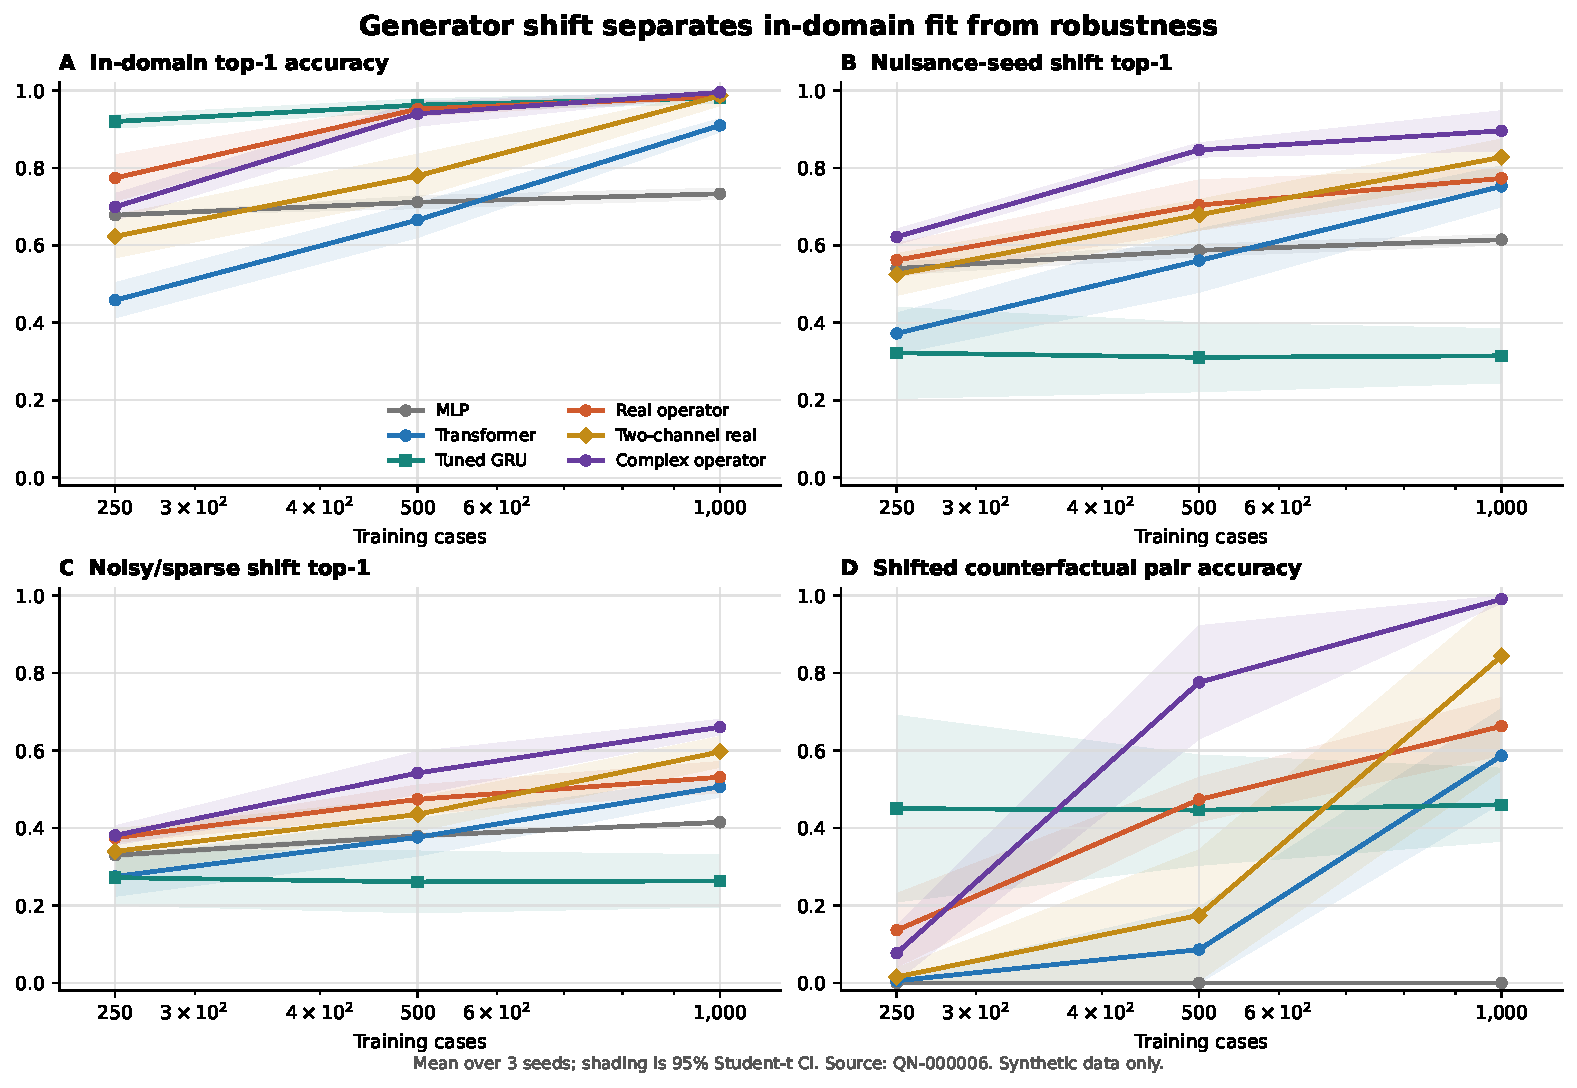
\includegraphics[width=0.98\linewidth]{figures/generator_shift_replication.pdf}
\caption{The stronger-control replication separates source-world fit from robustness. A tuned GRU is strongest at very low source data but collapses under the declared generator shifts; the complex operator becomes strongest under nuisance and noisy/sparse shift at 1,000 cases.}
\label{fig:generator_shift_replication}
\end{figure}

\subsection{Ambiguity, omitted labels, and hidden syndromes}
Irreducible ambiguity pairs present identical observations with two valid chronology labels. The ideal prediction assigns all mass equally to the twins, giving pair NLL log(2). This benchmark tests whether a differential remains calibrated when the label is unidentifiable. It is distinct from standard uncertainty on difficult but identifiable cases.

The omitted-disease task removes one label entirely during training and evaluates whether confidence or representation distance separates it from known cases. The hidden-syndrome task creates an unlabeled cross-factor signature and measures representation separation. Neither task claims disease discovery. High AUROC only shows that a synthetic construct lies away from known examples under a declared score.

\begin{figure}[t]
\centering
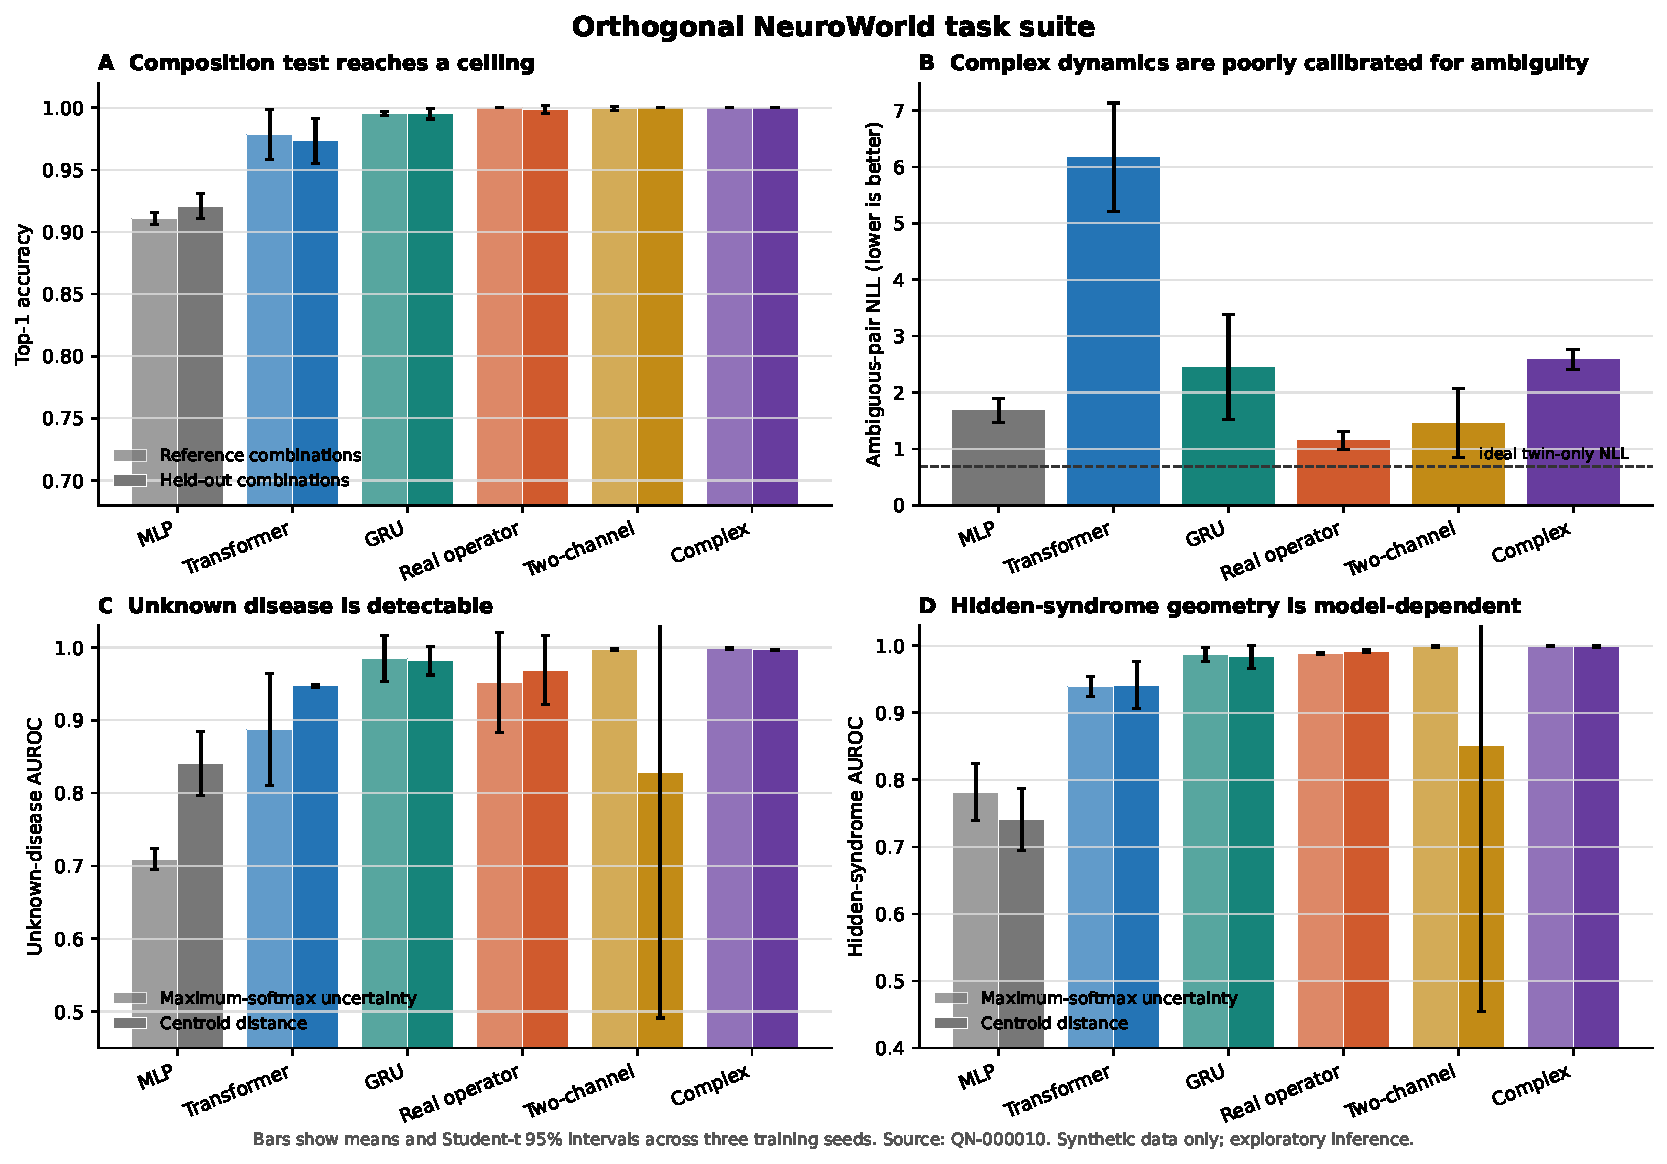
\includegraphics[width=0.98\linewidth]{figures/neuro_task_suite.pdf}
\caption{The orthogonal task suite separates composition, ambiguity, omitted-disease rejection, and hidden-syndrome representation tests. Success on one axis does not imply success on the others.}
\label{fig:neuro_task_suite}
\end{figure}

\subsection{Active evidence acquisition}
For active acquisition, the complete set of 40 binary outcomes exists but a policy reveals one at a time. Query costs are equal. Random order, fixed mutual-information order, and model-conditioned expected entropy reduction are evaluated from one to twelve queries. Accuracy AUC is the average top-1 across those budgets, not receiver-operating-characteristic area. This task excludes chronology twins so that a set-based query policy is not asked to infer event order from unordered acquisition.

The simulator does not model the causal dependence among requested tests, the semantics of asking a patient a question, or unequal cost and risk. It is a controlled partial-information benchmark. A clinically meaningful extension would need conditional outcome models, governed cost definitions, and prospective policy evaluation.

\subsection{Leakage and scope controls}
Train, validation, and test cases use disjoint random streams. Model selection never reads shifted test metrics. World seeds are held out before training. Counterfactual pairs are generated separately. The registry stores dataset fingerprints, configuration hashes, seeds, hardware/software environment, and result paths. One early asymmetric-input study is retained but superseded because only the MLP received demographic context; the corrected study equalizes inputs.

NeuroWorld remains a single simulator family built by the same project that proposes Q-Neuro. That is the largest external-validity limitation. Multiple seeds reduce sensitivity to one random template but do not create an independent scientific replication. The benchmark is best viewed as a causal wind tunnel: valuable for mechanism stress tests, insufficient for claims about real patients.
